\lstinputlisting[language=bash,basicstyle=\small]{python_codes/fieldstone_76/keywords}

\begin{center}
Code at \url{https://github.com/cedrict/fieldstone/tree/master/python_codes/fieldstone_76}
\end{center}

\par\noindent\rule{\textwidth}{0.4pt}

%%%%%%%%%%%%%%%%%%%%%%%%%%%%%%%%%%%%%%%%%%%%%%%%%%%%%%%%%%%%%%%%%%%%%%%%%%%%%%%%%%%%%%%%%%%%


This stone is an example of $Q_2\times P_{-1}$ implementation. 
The 2D $Q_2$ shape functions have been derived in Section~\ref{ss:q22d}
while the $P_{-1}$ shape functions are in Section~\ref{ss:lbfq2D}.
The $-1$ subscript indicates that the pressure field is linear, 
i.e. $p^h(x,y)=a+bx+cy$ inside the element, but discontinuous 
from an element to another. 
This poses a little problem in terms of exporting it to vtu (and plotting with paraview).
I then simply choose to export the value of the pressure in the middle of 
each element. 

I carry out two benchmarks and we recover for both a cubic convergence 
for the velocity error and a quadratic error convergence for the pressure.

%.......................................
\subsection*{Manufactured solution \#1}

The analytical solution originates in Lamichhane (2017) \cite{lami17}.
The velocity and pressure are given by
\begin{eqnarray}
u(x,y)&=&-2x^2y(2y-1)(x-1)^2(y-1) \\
v(x,y)&=& 2xy^2(2x-1)(x-1)(y-1)^2 \\
p(x,y)&=& x(1-x)(1-2y)
\end{eqnarray}
Boundary conditions are no-slip on all sides of the unit square. 
The corresponding body force terms are derived in Section~\ref{ss:mms11}. 

\begin{center}
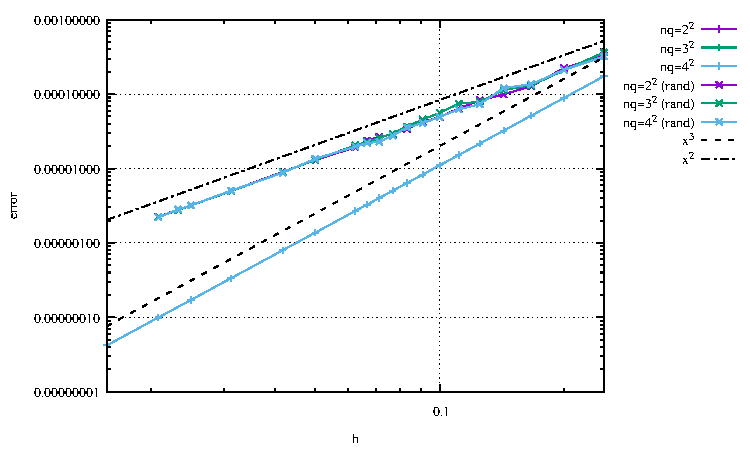
\includegraphics[width=7cm]{python_codes/fieldstone_76/results/mms1/errors_v}
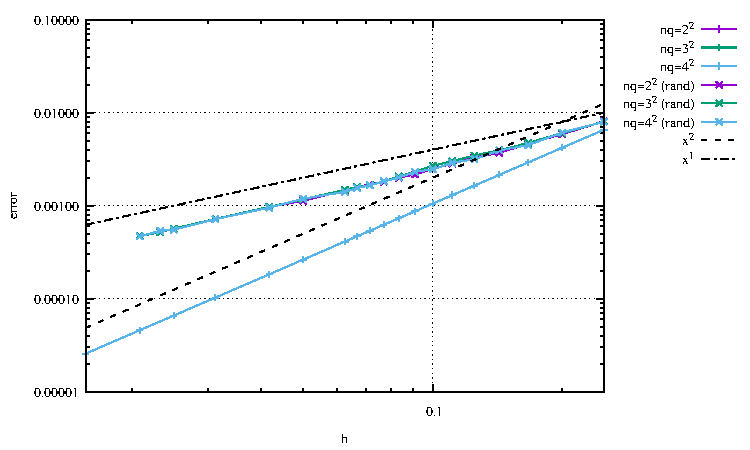
\includegraphics[width=7cm]{python_codes/fieldstone_76/results/mms1/errors_p}
\end{center}

\begin{center}
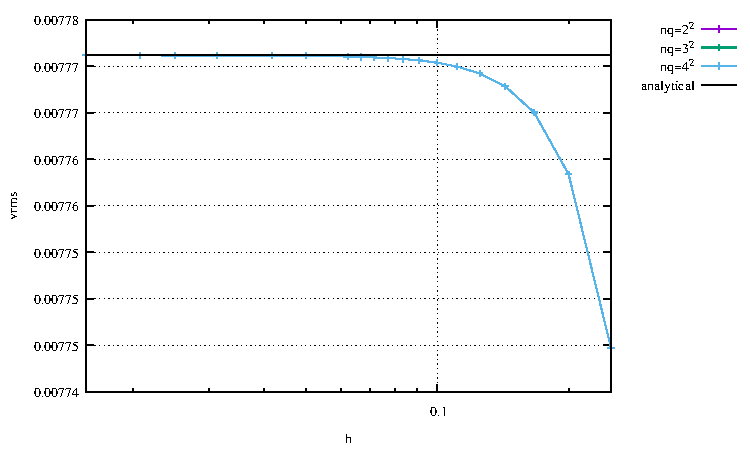
\includegraphics[width=9cm]{python_codes/fieldstone_76/results/mms1/vrms}
\end{center}

%.......................................
\subsection*{Manufactured solution \#2}

This is the second manufactured solution 
mentioned in Lamichhane \cite{lami17}. It is presented in Section~\ref{ss:mms2}.
It is for a unit square with $\eta=1$ and the smooth exact solution is
\begin{eqnarray}
u(x,y) &=& x+x^2 - 2xy+x^3 - 3xy^2 + x^2y \\
v(x,y) &=& -y-2xy+y^2 -3x^2y + y^3 - xy^2 \\
p(x,y) &=& xy+x+y+x^3y^2 - 4/3
\end{eqnarray}
Note that the pressure obeys $\int_{\Omega} p \; d\Omega = 0$. The analytical 
velocity is prescribed on the boundary of the domain. 


\begin{center}
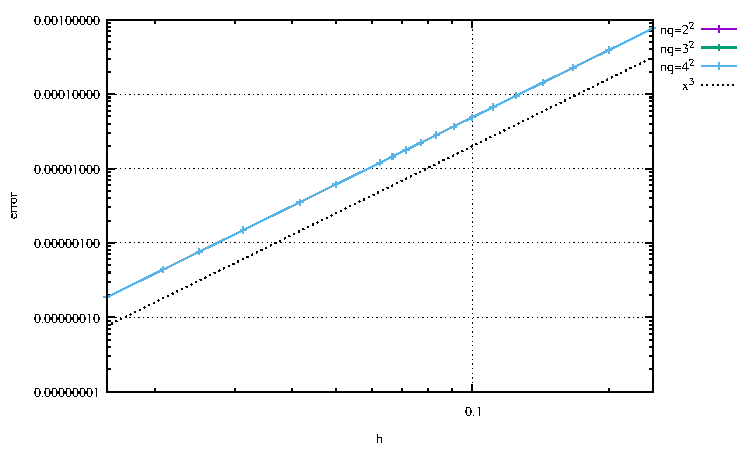
\includegraphics[width=7cm]{python_codes/fieldstone_76/results/mms2/errors_v}
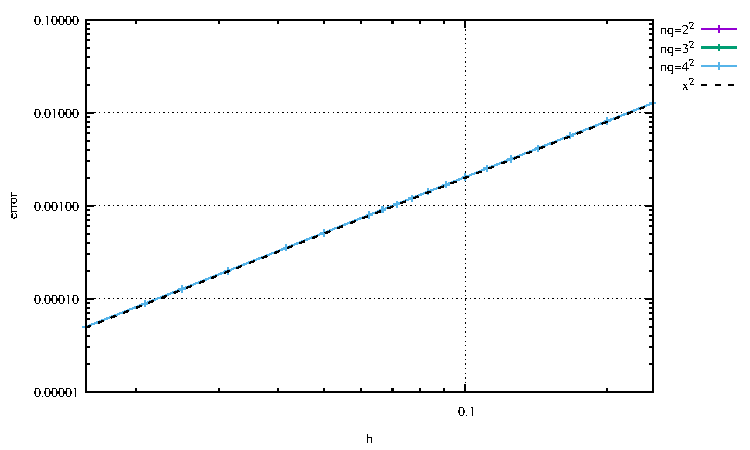
\includegraphics[width=7cm]{python_codes/fieldstone_76/results/mms2/errors_p}
\end{center}

\begin{center}
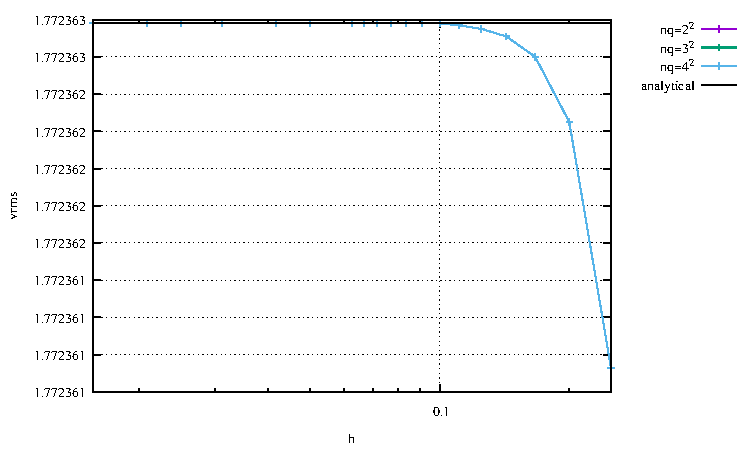
\includegraphics[width=9cm]{python_codes/fieldstone_76/results/mms2/vrms}
\end{center}


%.......................................
\subsection*{Instantaneous sinking block}

It is fully described in Section~\ref{ss:sinking_block}

\begin{center}
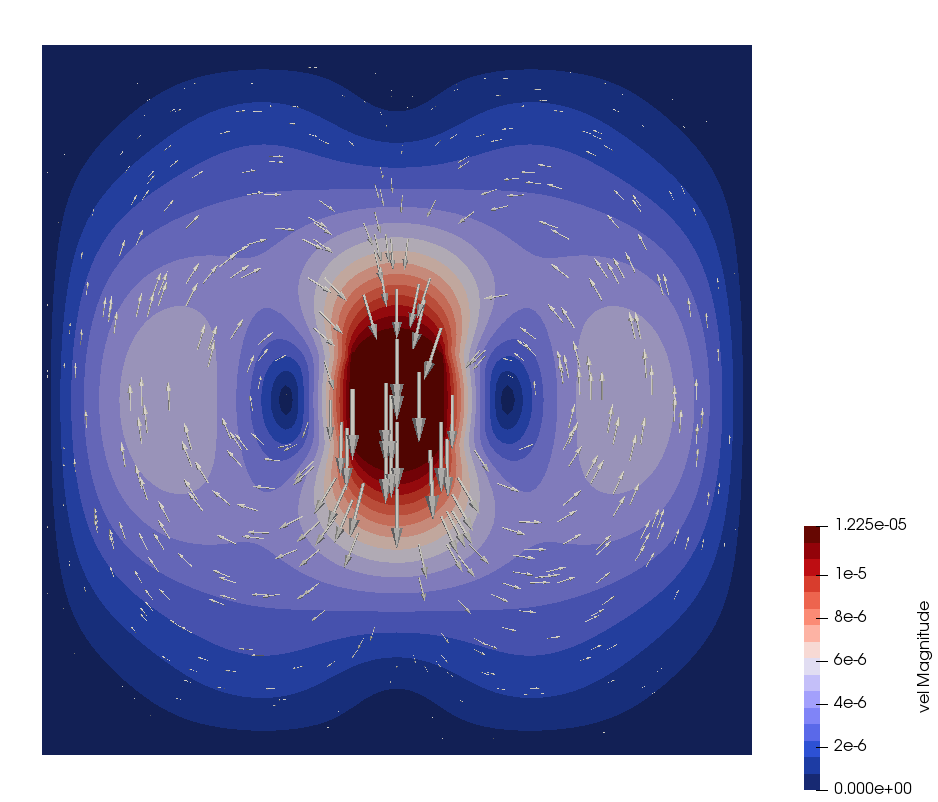
\includegraphics[width=7cm]{python_codes/fieldstone_76/results/block/vel}
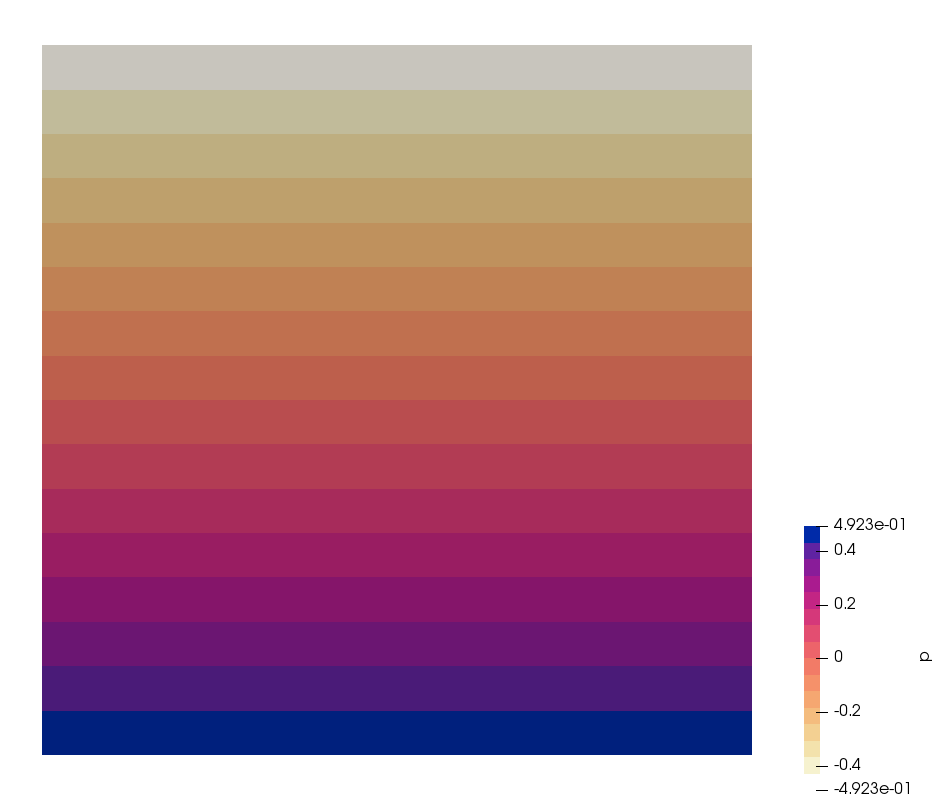
\includegraphics[width=7cm]{python_codes/fieldstone_76/results/block/press}
\end{center}


